\chapter{Test problems}

\section{Unconstrained programs}

\subsection{Univariate functions}

\section{Parabola}

\[
x^2+4x-10
\]

\begin{figure}[htb]
\begin{center}
\begin{small}
\include{parabola_1}
\end{small}
\end{center}
\caption{\texttt{parabola\_1} function}
\label{fig:parabola_1}
\end{figure}

\subsection{Multivariate functions}

\section{Bound constrained programs}

\subsection{Univariate functions}

\subsection{Multivariate functions}

\subsubsection{Hock}

The following functions are taken from \cite{HockSchi81}.
\[
f(x,y) = \frac{(x+1)^3}{3}+y
\]

\begin{figure}[htb]
\begin{center}
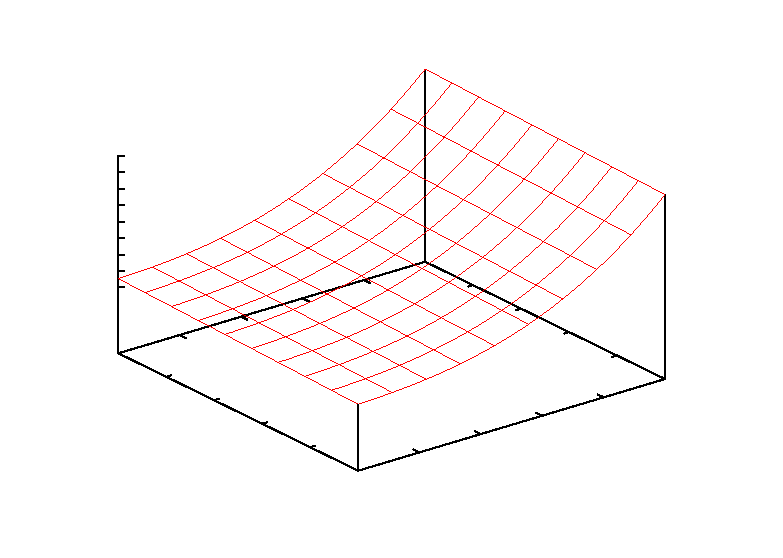
\includegraphics[width=0.7\textwidth]{pbr_t1_3}
\end{center}
\caption{\texttt{pbr t1 3} function}
\label{fig:pbr_t1_3}
\end{figure}

\section{Global optimization}

A set of functions are provided to test the capabilities to escape from local minimizer and identify a global minimizer.
These functions are characterized with the presence of several local minimizers, from where it is difficult for an algorithm to escape.

\subsection{Univariate functions}

\subsubsection{GSL E1}

This function has been taken from the GNU Scientific Library (\url{http://www.gnu.org/software/gsl}).
The function is considered to test the simulated annealing algorithm, under the name \texttt{E1}, and has the form
\[
f(x) = e^{-(x-1)^2}sin(8x)-0.89e^{-(x-1000)^2}
\]
Its graph is given in Figure~\ref{fig:gsl_e1}, and its definition is
\begin{verbatim}
double gsl_e1(double x)
\end{verbatim}
where $x$ is the point where we want to evaluate the function.
We denote if by \verb|gsl e1|.
The optimal value is $f^* = -0.87287$, attained at $x^* = 1.36312999$.
The function has also a local minimizer at $x = 0.60146196$, for an objective value $f = -0.84893$.

\begin{figure}[htb]
\begin{center}
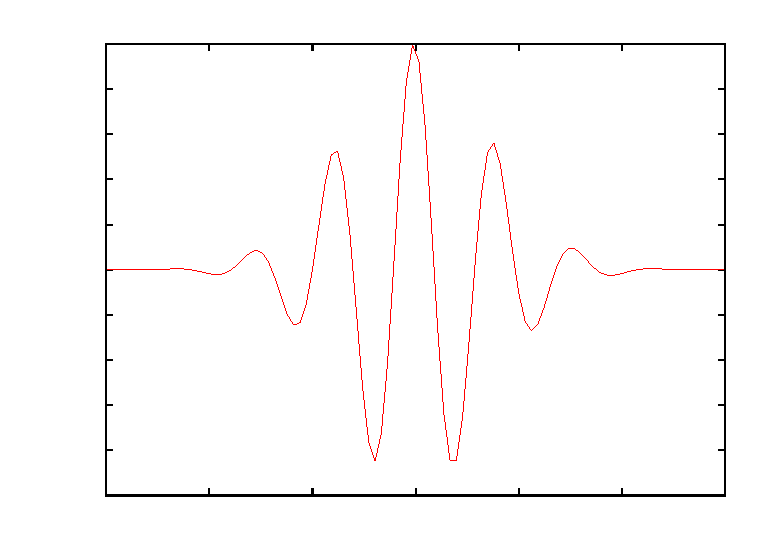
\includegraphics[width=0.7\textwidth]{gsl_e1}
\end{center}
\caption{\texttt{gsl e1} function}
\label{fig:gsl_e1}
\end{figure}

\subsection{Multivariate functions}

Ackley's function
\begin{equation}
f(x,y) = -20 e^{-0.2 \sqrt{0.5(x^2+y^2)}}-e^{0.5(\cos(2\pi x)+\cos(2\pi y))}+e+20
\end{equation}
The global minimizer is $(0,0)$, with the corresponding objective value $f(0,0) = 0$.
